\section{Architecture de l’Internet des objets}

\begin{figure}[h]
	\centering
    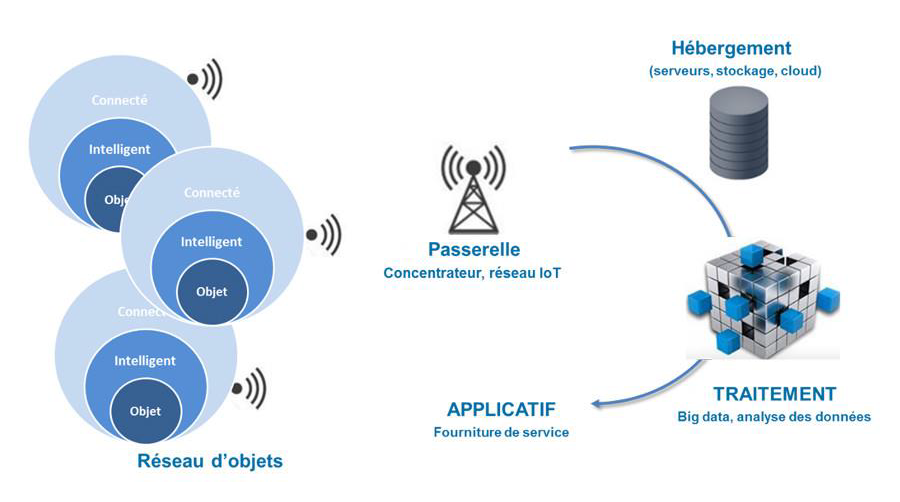
\includegraphics[scale=0.5]{img/part1/2.2}
    \caption{Architecture de l’Internet des objets}
\end{figure}

Précisons le rôle des différents processus présentés sur ce schéma :
\begin{itemize}[label=\textbullet]
\item \textbf{Capter:} désigne l’action de transformer une grandeur physique analogique en un signal numérique.
\item \textbf{Concentrer:} permet d’interfacer un réseau spécialisé d’objet à un réseau IP standard (e.g. WiFi) ou des dispositifs grand public.
\item \textbf{Stocker:} qualifie le fait d’agréger des données brutes, produites en temps réel, méta taguées, arrivant de façon non prédictible.
\item \textbf{Présenter:} indique la capacité de restituer les informations de façon compréhensible par l’Homme, tout en lui offrant un moyen d’agir et/ou d’interagir.
\end{itemize}

Deux autres processus n’apparaissent pas sur le schéma, car ils sont à la fois transverves et omniprésents :
\begin{itemize}[label=\textbullet]
\item \textbf{Le traitement des données:} est un processus qui peut intervenir à tous les niveaux de la chaîne, depuis la capture de l’information jusqu’à sa restitution. Une stratégie pertinente, et commune quand on parle d’Internet des objets, consiste à stocker l’information dans sa forme intégrale. On collecte de manière exhaustive, « big data », sans préjuger des traitements qu’on fera subir aux données. Cette stratégie est possible aujourd’hui grâce à des architectures distribuées type NoSQL, capables d’emmagasiner de grandes quantités d’information tout en offrant la possibilité de réaliser des traitements complexes en leur sein (Map/Reduce par exemple).
\item \textbf{La transmission des données:} est un processus qui intervient à tous les niveaux de la chaîne.
\end{itemize}